

\section{Why we need MRE}

% 
% \frame{\titlepage}

\begin{frame}[t]{Why do we need MRE?}

% \vspace{-\baselineskip}
% \begin{center}
% 	\define{Environmental monitoring problems} are of great \\ importance in many practical applications.
% \end{center}

% \vspace{.5\baselineskip}

\begin{columns}[T]
\column{.4\textwidth}
  \begin{itemize}
    \item<2-> diseased tissue changes mechanical
    \item<3-> low tech: palpation
    \item<4-> higher tech: ultrasound
    \item<5-> highest tech: MRE
    \item<6-> for deep tissue and brains, but non-invasive
  \end{itemize}
\column{.6\textwidth}

 	\vspace{-0.5cm}
	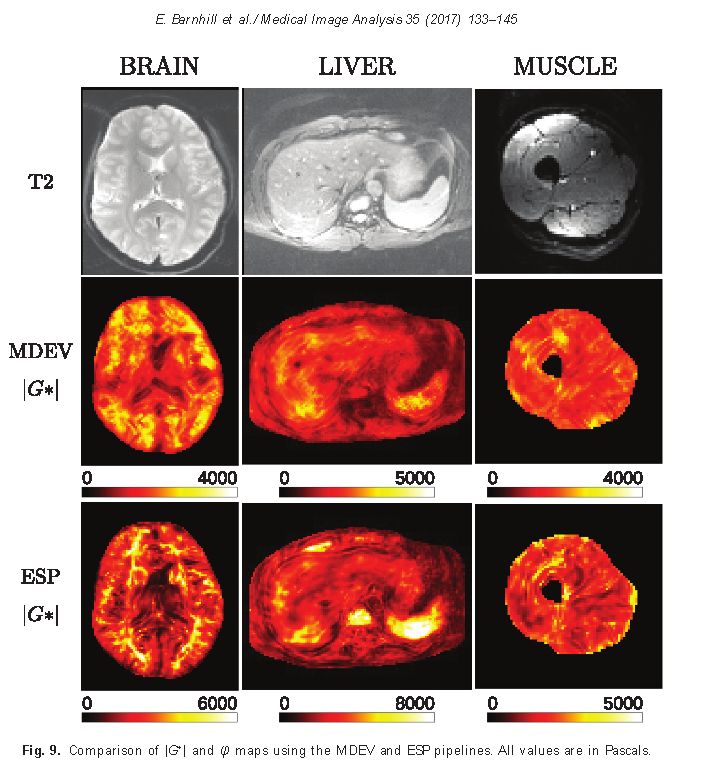
\includegraphics[width=\textwidth]{Images/Elasto-Tissue.pdf}

\end{columns}

\end{frame}



\begin{frame}{How does the measuring process work?}

\begin{figure}
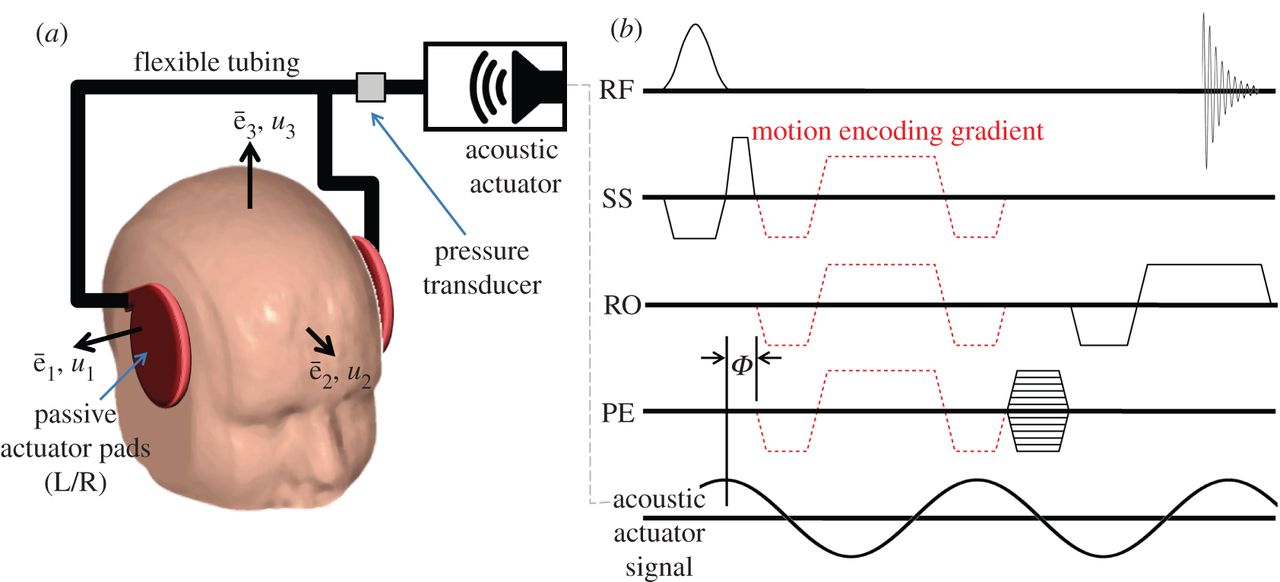
\includegraphics[width=0.9\textwidth]{Images/experiment.jpg}
\centering\end{figure}

\begin{itemize}
 \item<2-> 3 spatial directions $\times$ 8 time steps $\times$ 3 frequencies
 \item<3-> 72 times longer per pixel than MRI 
\end{itemize}

\end{frame}

\section{Data Reconstruction and current Problems}

\begin{frame}{How does the tissue movement relate to stiffness?}


\begin{itemize}
 \item<2-> Navier-Lam\'{e} equation:
 \begin{equation}
 \sum_ j \partial_j \kl{ \mu \kl{ \partial_j u_i + \partial_i u_j}} + \partial_i \kl{\lambda \partial_j u_j} = \rho \ddot{u}_i
\end{equation}
\item<3-> time harmonic and small bulk wave
 \begin{equation}
 \nabla(\bm{\mu}  \cdot \epsilon) = -\rho \omega^2 \mathbf{u} \quad \text{with} \quad \epsilon_{ij} = \partial_j u_i + \partial_i u_j
\end{equation}
 \item<4-> discretize the equation
 \begin{equation}
 \ekl{\nabla\cdot\epsilon + \epsilon\nabla} \bm{\mu} = -\rho \omega^2 \mathbf{u}
\end{equation}
 \item<5-> matrix inversion relies on correct knowledge of $\mathbf{u}^{'}$, and $\mathbf{u}^{''}$\\
 $\rightarrow$ noise can completely screw up the derivatives
\end{itemize}

\end{frame}


\begin{frame}{Noisy displacement field}

\begin{figure}
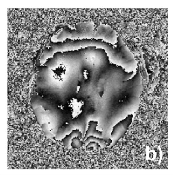
\includegraphics[width=0.5\textwidth]{Images/noisyBrain.png}
\caption{b) The human brain}
\centering\end{figure}

\end{frame}


\begin{frame}{Wavelet Denoising}

\begin{itemize}
 \item<2-> $\mathbf{u}(\mathbf{x},t)$ is piece-wise (very) smooth $\rightarrow$ sparse in wavelet domain
 \item<4-> in 2d: anisotropic structure $\rightarrow$ shearlets
\end{itemize}

\only<1-2>{
\vspace{5.1cm}
}

\only<3-4>{
\visible<3->{
\begin{figure}
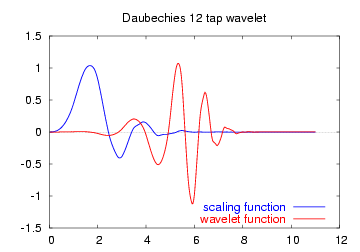
\includegraphics[width=0.5\textwidth]{Images/Daubechies.png}
\centering\end{figure}
}
}

\only<5>{
\vspace{0.95cm}
\begin{figure}
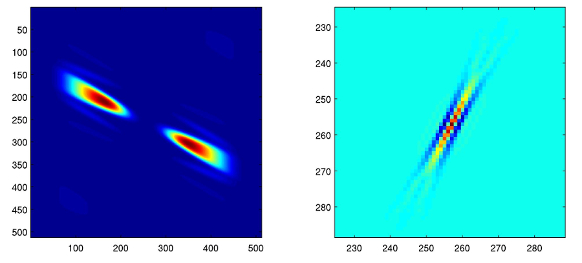
\includegraphics[width=0.6\textwidth]{Images/shearlet.jpeg}
\centering\end{figure}
}

\only<6->{
\vspace{1cm}
\begin{block}{Wavelet Denoising:}
 \begin{align}
  u^* &= \underset{u}{\text{argmin}}~\nkl{u_{\text{meas}} - u}^2_2 + \lambda \nkl{W u}_0 \\
      &= W^{\dagger} H\kl{W u_{\text{meas}}; \lambda}
 \end{align}
\end{block}
\vspace{1cm}
}


\end{frame}


% \begin{frame}		\frametitle{Data reconstruction}
% 
% 
% \begin{align}
%  \mathbf{u} &= \mathbf{u}(\xb,t) \\
%  \mu &=
% \end{align}
% 
% 
% 
% \begin{equation}
%  A\mathbf{\mu} = \mathbf{b}
% \end{equation}
% 
% 
% \end{frame}
% 
% \begin{frame}{Underdetermined System}
% 
% 
% \begin{itemize}
%  \item differential equation --> inverse problem
%  \item Problem underdetermined, we need boundary values
%  \item Problem: some regions are close to nodes --> no movement
%  \item Solution: Multi frequency inversion
%  \item Problem: Need to reconstruct the derivatives
%  \item motion encoding gradient
%  \item MRI measurement in 3 spatial directions and 8 time steps
% \end{itemize}
% 
% \begin{itemize}
%  \item MRI measurement in 3 spatial directions and 8 time steps and 3 frequencies --> 72 times MRI overhead
%  \item --> reduced resolution
% \end{itemize}
% 
% \begin{itemize}
% 
%  \item Problem: Need to reconstruct the derivatives
%  \item slight noise can lead to totally wrong derivatives --> inversion is useless
%  \item MRI measurement in 3 spatial directions and 8 time steps
% \end{itemize}
% 
% \end{frame}
% 
% \section{Denoising Techniques}


\begin{frame}
 
 \begin{figure}
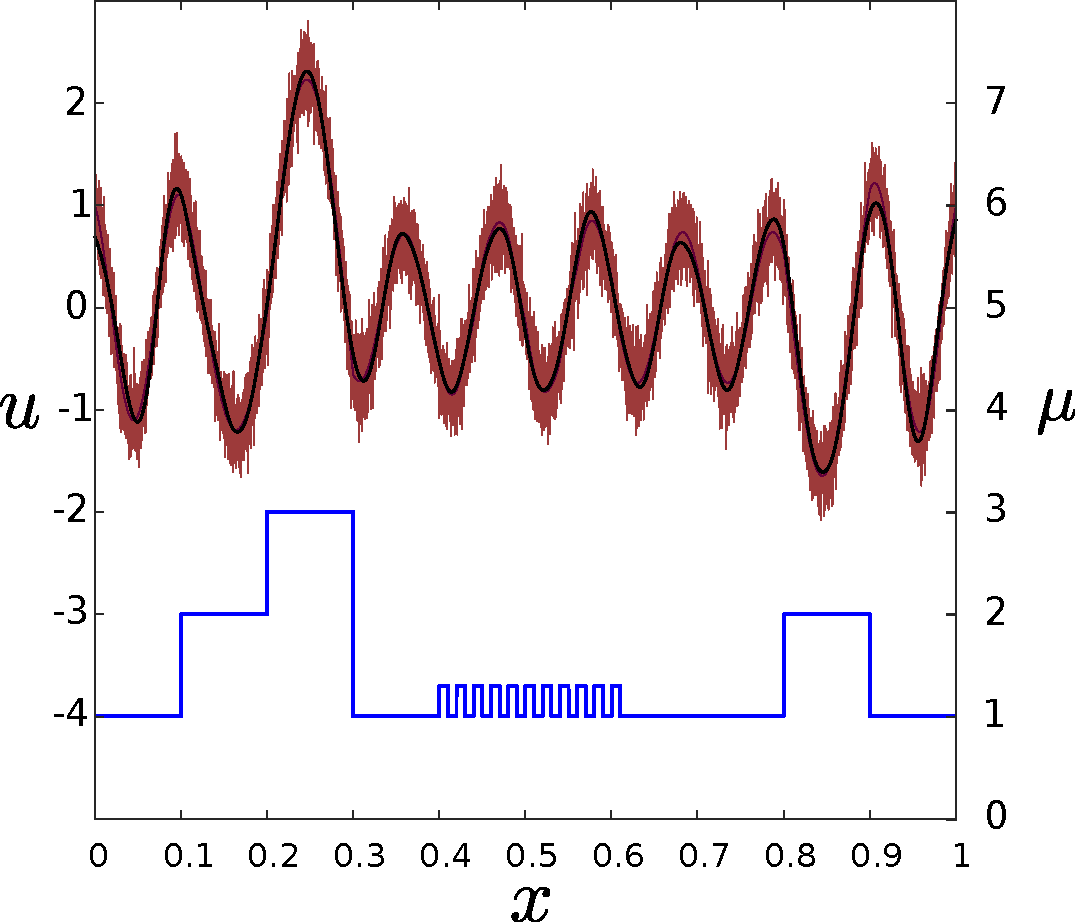
\includegraphics[width=0.7\textwidth]{Images/waveDenoising.pdf}
\centering
\caption{Shear parameter, displacement and noise in 1d}
\end{figure}
\end{frame}

\begin{frame}
 \begin{figure}
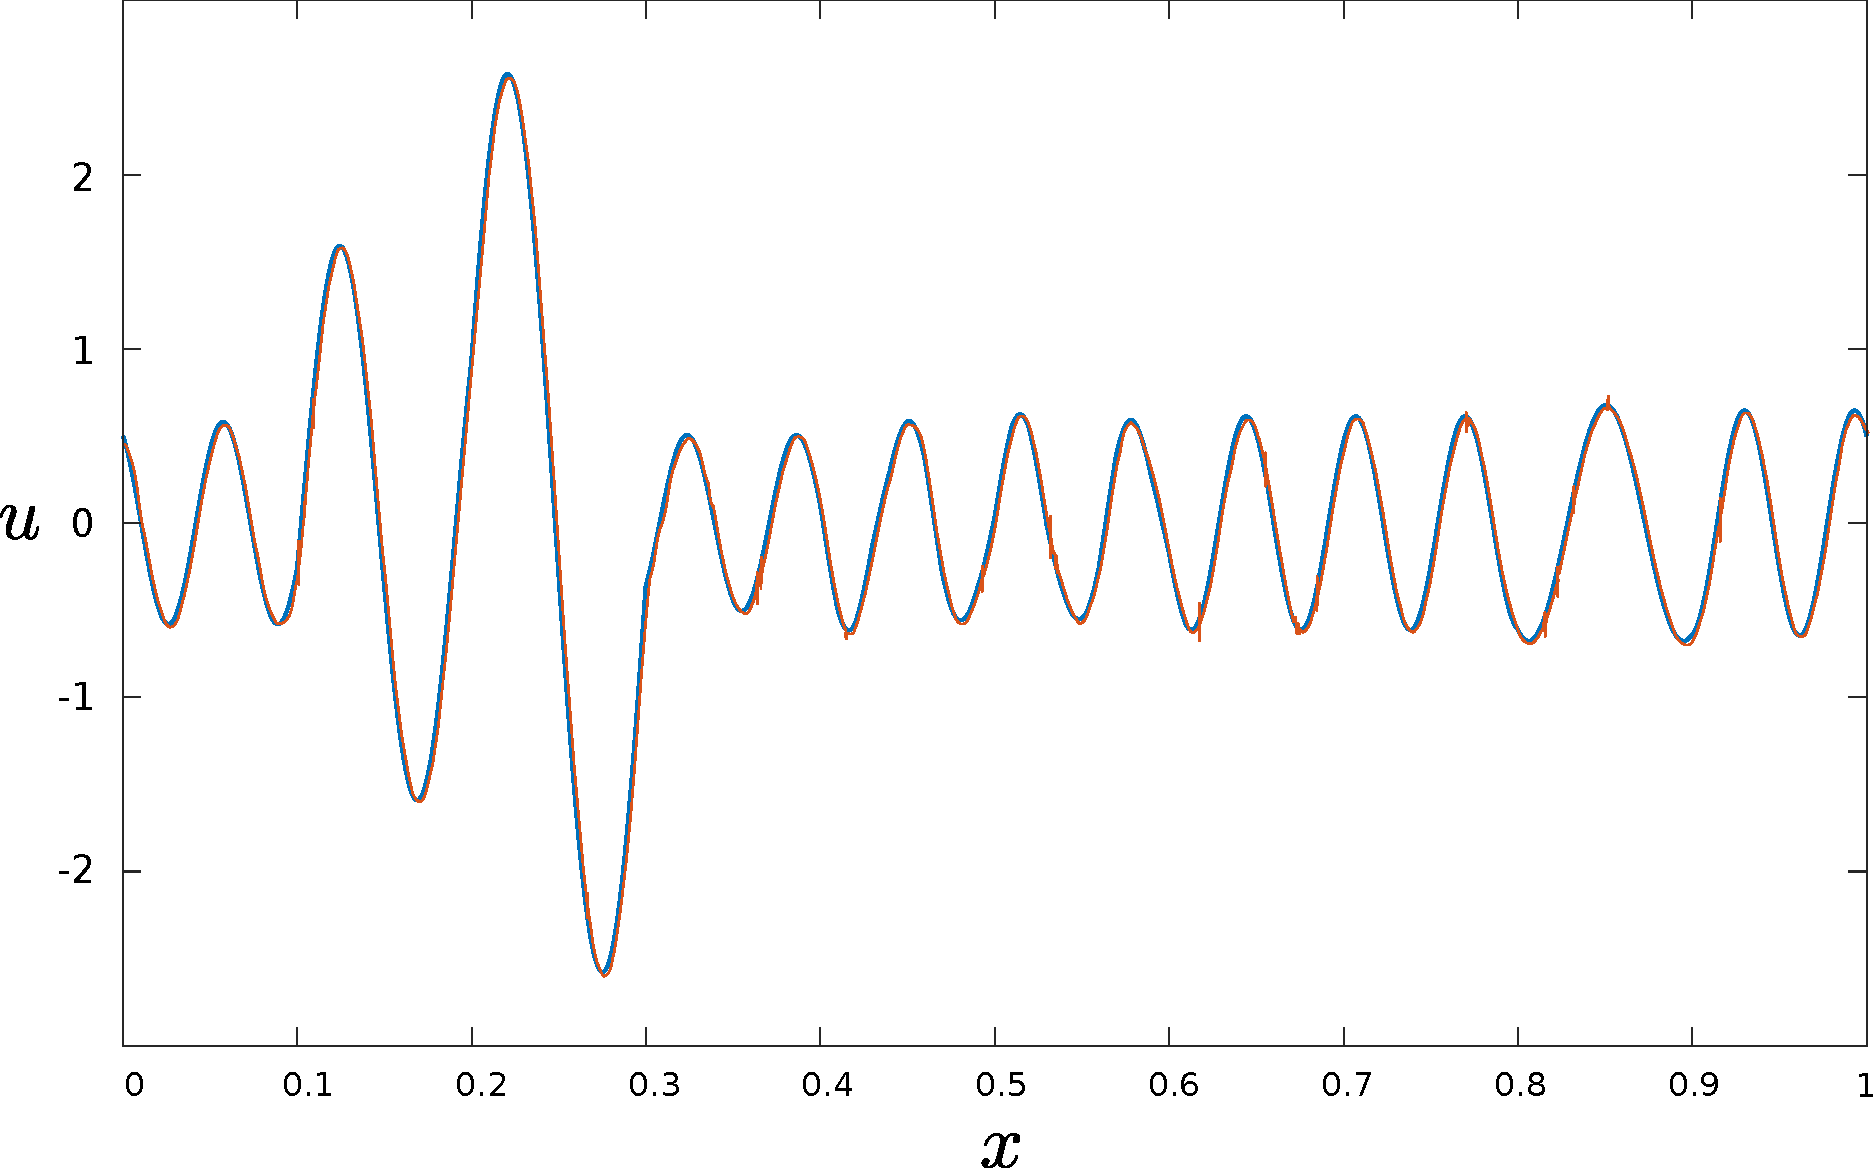
\includegraphics[width=0.8\textwidth]{Images/littleSpikes.pdf}
\caption{Reconstructed with Daubeshies10-wavelets and threshold of $0.01*\max_i(u_i)$}
\centering
\end{figure}
\end{frame}

\begin{frame}
 \begin{figure}
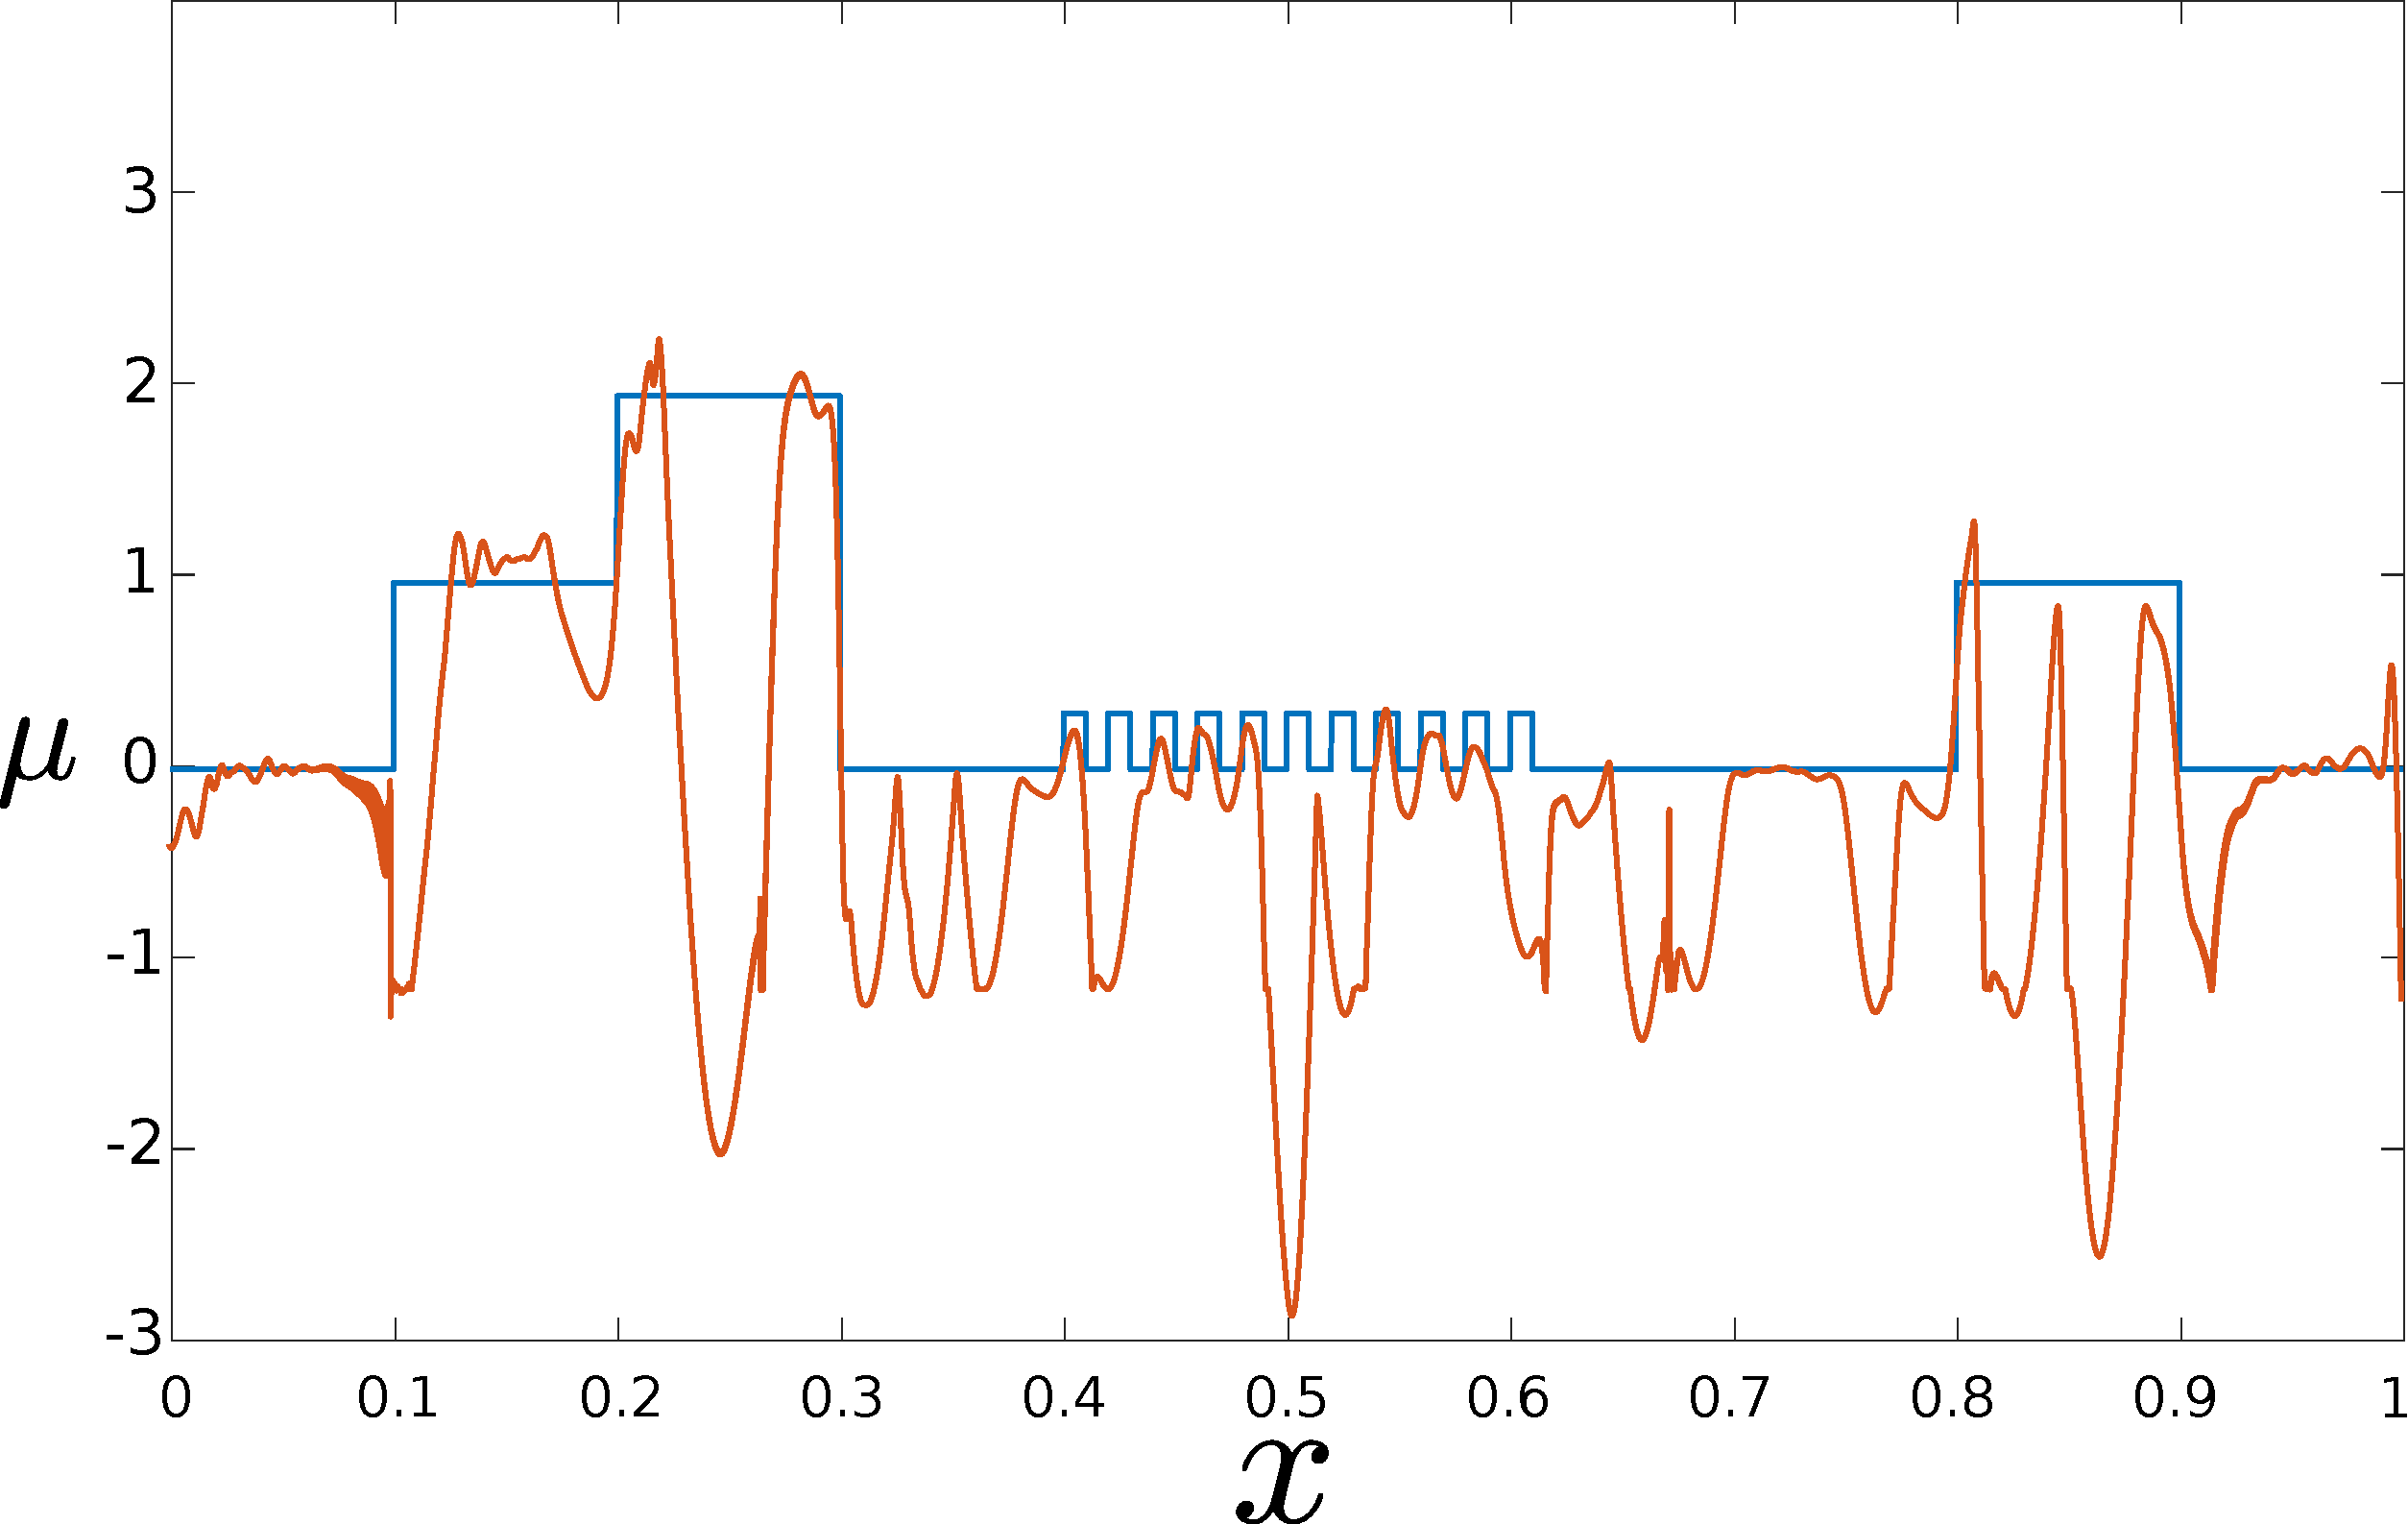
\includegraphics[width=0.8\textwidth]{Images/muCorrupted.pdf}
\centering
\caption{Original and reconstructed shear parameter $\mu$.}
\end{figure}
\end{frame}

\begin{frame}
 \begin{figure}
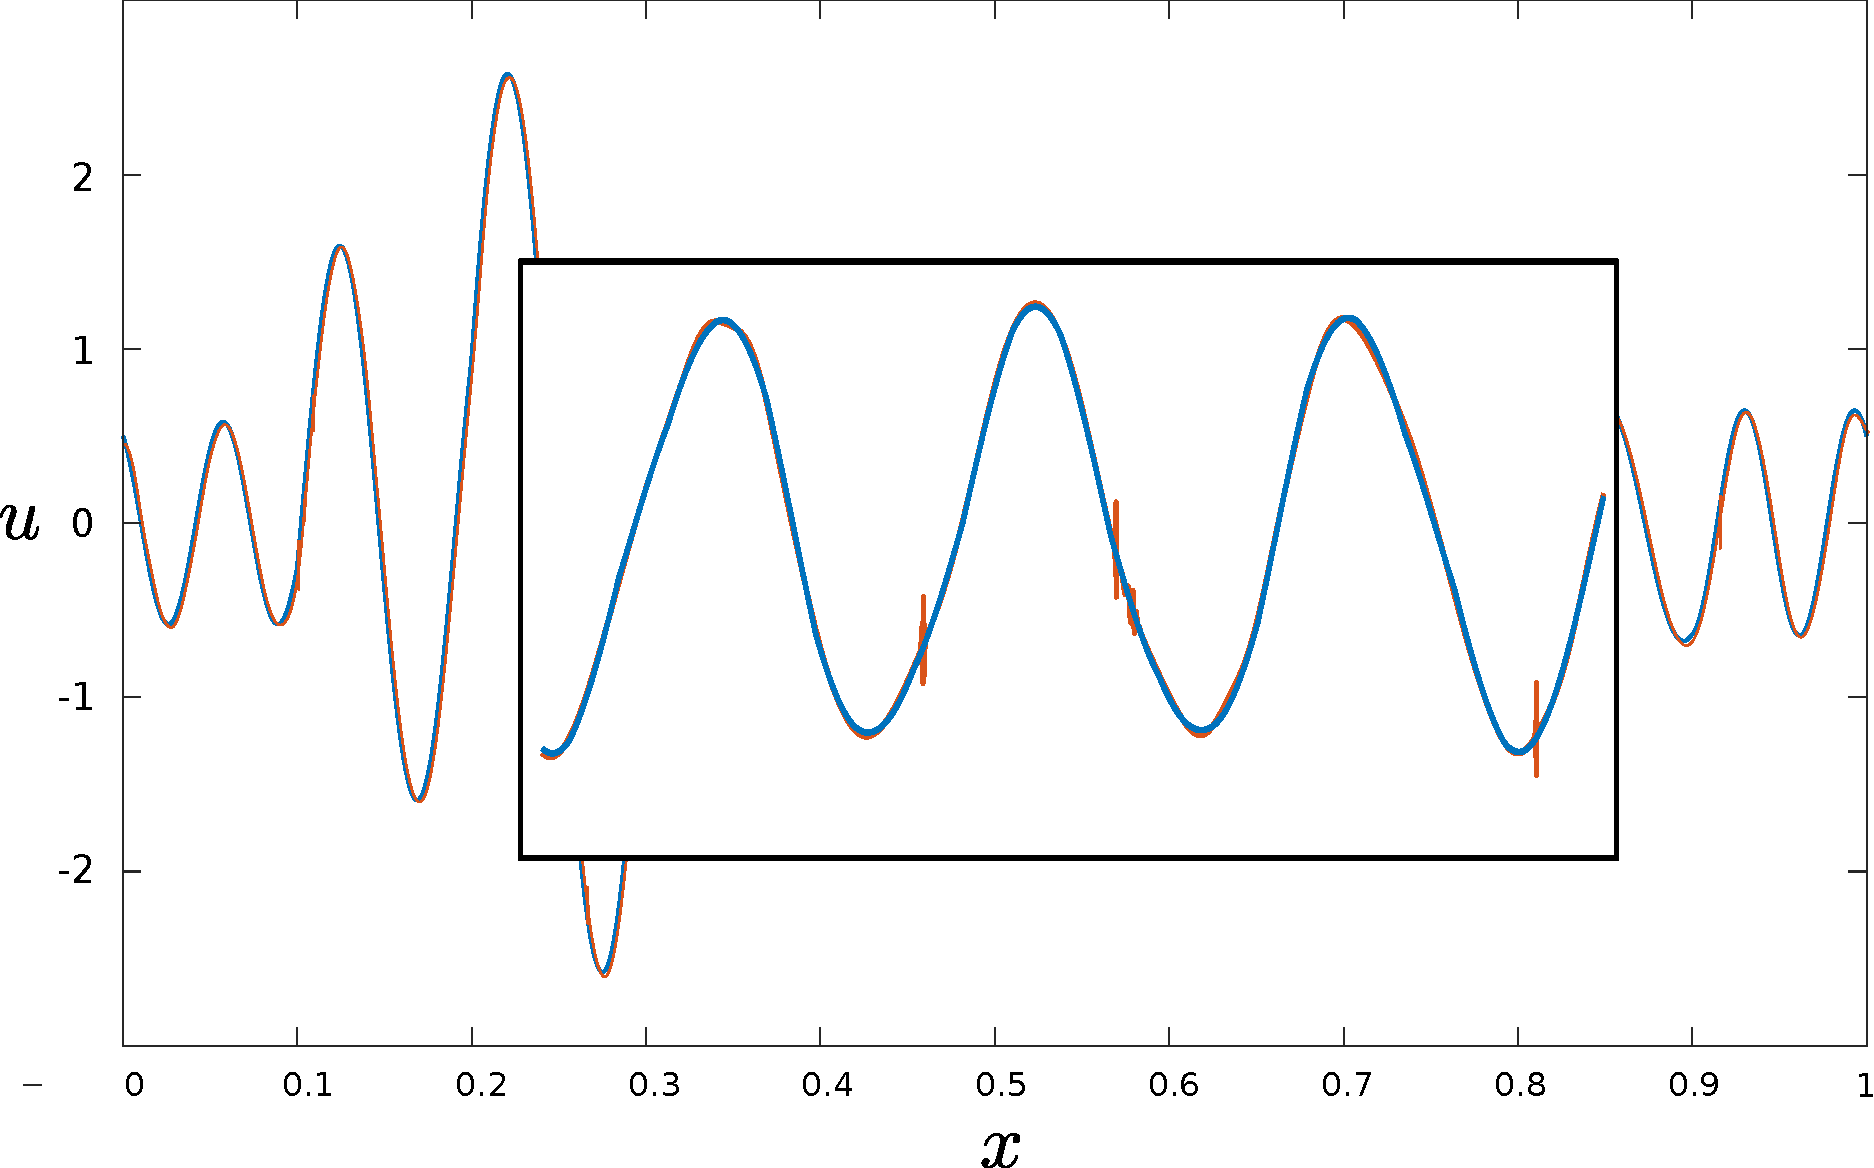
\includegraphics[width=0.8\textwidth]{Images/littleSpikesClose.pdf}
\caption{First derivative of original and denoised displacement $u$. Close-up reveals noise residuals on a fine scale.}
\centering\end{figure}
\end{frame}

\begin{frame}
 \begin{figure}
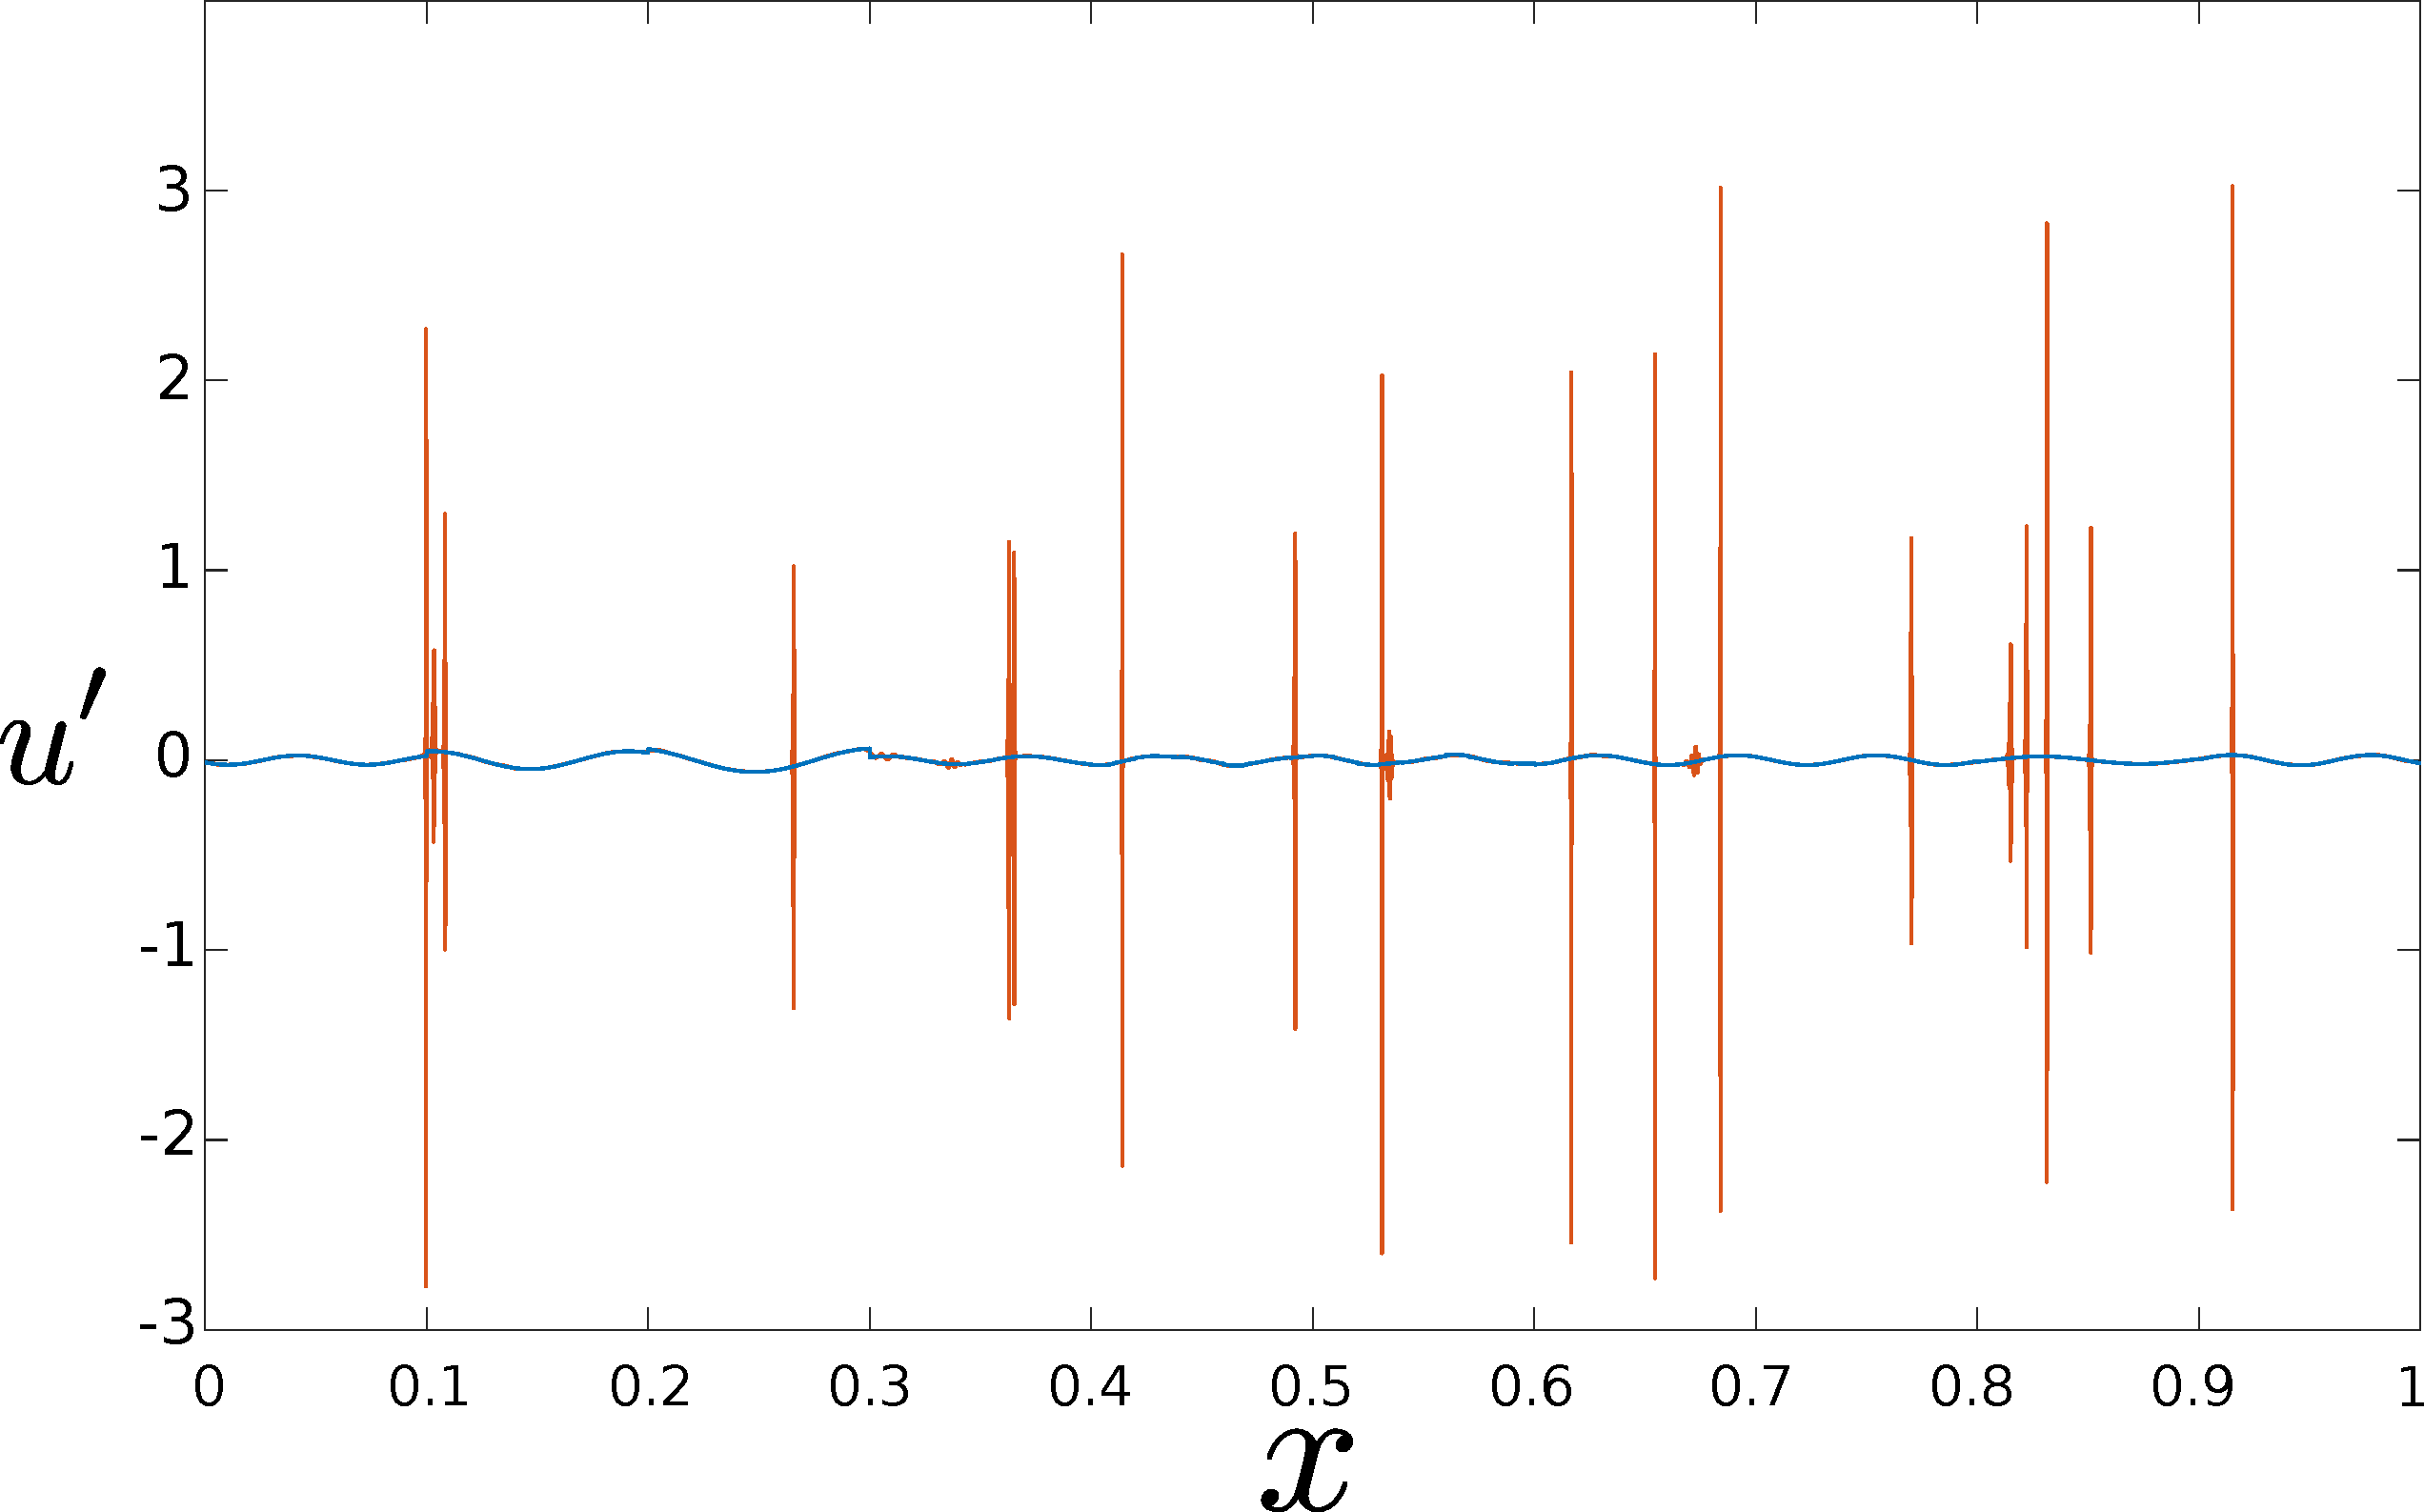
\includegraphics[width=0.8\textwidth]{Images/derivative.pdf}
\caption{First derivative of original and denoised displacement $u$. Fine scale noise dominates the first (and subsequent) derivatives.}
\centering\end{figure}
\end{frame}


\section{First Experiments}


\begin{frame}		\frametitle{Our plan of work}

\begin{itemize}
 \item Do simuations in 1d: wavelets
 \item Do simulations in 2d: wavelets, shearlets
 \item 
\end{itemize}

\begin{itemize}
 \item Problem: Need to reconstruct the derivatives
 \item slight noise can lead to totally wrong derivatives --> inversion is useless
 \item MRI measurement in 3 spatial directions and 8 time steps --> 
\end{itemize}

\end{frame}

\section{What comes next}


\begin{frame}		\frametitle{What would be nice results}

\begin{itemize}
 \item Have better resolution of the stiffness map
 \item Have clinically useful values, at the moment to varying
 \item Have shorter acquisition times per pixel
\end{itemize}

\begin{itemize}
 \item Problem: Need to reconstruct the derivatives
 \item slight noise can lead to totally wrong derivatives --> inversion is useless
 \item MRI measurement in 3 spatial directions and 8 time steps --> 
\end{itemize}

\end{frame}





 